
\begin{comment}

    Introduction
     - What are approximate solutions
     - Why and what does it try to solve
       • Continuos or large state and action spaces.
    
    Stochastic gradient and semi gradient

    Linear methods
     - poly
     - fourier
     - tile-coding
     - rbf
     - maybe more stuff, but I'll probably not try anything else

    Non-linear methods
     - ANN
     - LSTD
     - Memory based
     - Kernel based

    Eligibility traces (maybe not)

    Policy gradient

    Value function based example
     - continuos state space, but discreet action space
     - pole
     - something else I haven't written yet, but the same as the previous example so we can compare the two

    Policy gradient based example
     - continuos state and action space
     - same model as above

\end{comment}

\section{Approximate solutions}
\label{sec:approximate_solutions}

Up until now all methods discussed used tables to store the learned value functions and policies. However these methods are not practical for many of the tasks where \acrfull{rl} is applied due these having large and continuos state spaces. 

The problem with large state spaces is not just the memory needed to store the table, but also the time and amount of data needed to fill in these tables accurately. For many of these tasks the states encountered will never have been seen before, thus to make decisions it is necessary to generalize from previous encounters with different states that are similar to the current one. In other words the key issue is that of \emph{generalization}. How can experience with a limited subset of states be generalized to produce a good approximation of a much larger subset?

Fortunately, generalization from examples has been extensively studied, and thus the problem to be solved is combining existing generalization methods with \gls{rl} methods. The type of generalization methods required are often called \emph{function approximation} because it take in samples of the target function and creates an approximation of the entire function.


\subsection{Stochastic Gradient Decent methods}
\label{sec:stochastic_gradient_decent_methods}
\acrfull{sgd} methods are a class of function approximation learning methods well suited for the field of \acrfull{rl}. In these methods the weight vector is a real valued column vector with a fixed number of elements, $\nd{w}=\left (w_1, w_2, ..., w_n \right )^T$, and the approximate function $\hat{v}\left(s, \nd{w}\right)$ is differentiable w.r.t. all weights in $\nd{w}$ at all states $s \in \mathcal{S}$.

The goal is to update the weights in $\nd{w}$ after each observation such that the approximate function $\hat{v}\left(s, \nd{w}\right)$ better approximates the real function $v_{\pi}\left(s\right)$. This can be done by updating the weights in the direction that would reduce the error the most. A definition of this error is thus needed, one possibility is to use the \emph{Mean Squared Value Error} $\overline{\text{VE}}$ shown below \cite{sutton2018reinforcement}.

\begin{equation}
    \overline{\text{VE}}\left(\nd{w}\right) \doteq  \sum_{s\in S} \mu(s) \left[v_{\pi}\left(s\right) - \hat{v}\left(s, \nd{w}\right) \right]^2
\end{equation}

Here is $\mu(s)$ the \emph{state weight distribution}, it is used to indicate which states are more important. This may be necessary since the number of weights in $\nd{w}$ can be significantly smaller than the total number of states, thus prioritizing certain states may be needed.

The following update rule for the weights in $\nd{w}$ may be defined, using $\overline{\text{VE}}$ and assuming the probability for each state to appear is uniformly distributed.

\begin{align}
  \nd{w}_{t+1} &\doteq \nd{w}_t - \frac{1}{2} \alpha \nabla \left[v_{\pi}\left(S_t\right) - \hat{v}\left(S_t, \nd{w}\right) \right]^2 \\
  &= \nd{w}_t + \alpha \left[v_{\pi}\left(S_t\right) - \hat{v}\left(S_t, \nd{w}\right) \right] \nabla \hat{v}\left(S_t, \nd{w}\right)
  \label{eq:w_update}
\end{align}

\acrshort{sgd} methods are \emph{Gradient Decent} because the updates to the weight vector $\nd{w}$ are proportional to the negative gradient of each sample's error. This is the direction where error falls the fastest. Gradient decent methods are called \emph{stochastic} when the updates are done using single samples which may have been selected stochastically. In these cases the updates apply small corrections to the weights and over the course of may iterations it has the effect of reducing the error.

The real value function $v_{\pi}\left(s\right)$ is in practice often not known. Thus the \gls{sgd} may be generalized by substituting it with $U_t$. This not the true value, $v_{\pi}\left(S_t\right)$, but an approximation of it. It may for example be a noise-corrupted version of $v_{\pi}\left(S_t\right)$, or one of the bootstrapping targets for $\hat{v}$ (eg. $G_t$, $G_{t:t+n}$, etc).

\begin{equation}
  \nd{w}_{t+1} = \nd{w}_t + \alpha \left[U_t - \hat{v}\left(S_t, \nd{w}\right) \right] \nabla \hat{v}\left(S_t, \nd{w}\right)
  \label{eq:vpist_w_update}
\end{equation}


\subsection{Artificial Neural Networks}
\Acrfullpl{ann} are widely used for nonlinear function approximation in the field of machine learning and beyond. Deeply-layered \acrshortpl{ann} have successfully been used in the Reinforcement Learning to solve complex problems. 

An \acrshort{ann} consists of interconnected units which have a similar function to a neuron in a nervous system. Figure~\ref{fig:ann} shows a simple \acrfull{ffnn} with three inputs, three hidden layers and two outputs. The layers are connected to with links, with each link having a real-valued weight associated with it. The links are comparable to synaptic connections in a nervous system and the weight are roughly comparable to the efficacy of the synaptic connections.

Each one of the units computes its output by first calculating a weighted sum of the inputs and then applies a non-linear function to the result. This non-linear function is called an \emph{activation function}. The activation function is often S-shaped, or sigmoid, for example a hyperbolic tangent, but sometimes a rectifier non-linearity, $f(x)=\max(0, x)$, or step function are also used. It's often useful for different layers to have different types of activation functions.

A \acrshort{ffnn} with no hidden layers is only able to approximate linear functions, however if a single hidden layer with a large enough number sigmoid elements is added, then any continuos function may be approximated within a range of input values with any degree of accuracy\cite{cybenko1989approximation}. This is also true for other non-linear functions that satisfy certain conditions, however non-linearity is essential. Non-linear activation functions are equivalent to a network without hidden layers, since linear functions of linear functions are linear. 

Even though a single hidden layer is enough to approximate any function, both practice and theory show that for the complex functions needed in many artificial intelligent tasks it's often easier or may even require abstractions which are hierarchical compositions of many layers of
lower-level abstractions, that is, abstractions produced by deep architectures such as \acrshortpl{ann} with many hidden layers \cite{bengio2009learning,sutton2018reinforcement}.

\begin{figure}[ht]			
	\centering
	

\tikzset{every picture/.style={line width=0.75pt}} %set default line width to 0.75pt        

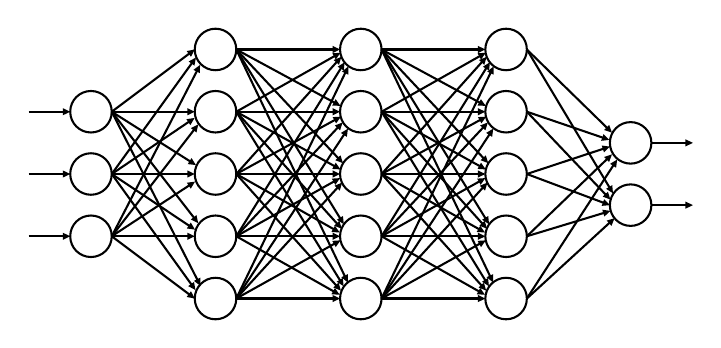
\begin{tikzpicture}[x=0.75pt,y=0.75pt,yscale=-1,xscale=1]
%uncomment if require: \path (0,415); %set diagram left start at 0, and has height of 415

%Shape: Circle [id:dp8746307842238439] 
\draw   (20.67,42) .. controls (20.67,36.48) and (25.14,32) .. (30.67,32) .. controls (36.19,32) and (40.67,36.48) .. (40.67,42) .. controls (40.67,47.52) and (36.19,52) .. (30.67,52) .. controls (25.14,52) and (20.67,47.52) .. (20.67,42) -- cycle ;
%Shape: Circle [id:dp913657480337059] 
\draw   (20.67,72) .. controls (20.67,66.48) and (25.14,62) .. (30.67,62) .. controls (36.19,62) and (40.67,66.48) .. (40.67,72) .. controls (40.67,77.52) and (36.19,82) .. (30.67,82) .. controls (25.14,82) and (20.67,77.52) .. (20.67,72) -- cycle ;
%Shape: Circle [id:dp5246690463386483] 
\draw   (20.67,102) .. controls (20.67,96.48) and (25.14,92) .. (30.67,92) .. controls (36.19,92) and (40.67,96.48) .. (40.67,102) .. controls (40.67,107.52) and (36.19,112) .. (30.67,112) .. controls (25.14,112) and (20.67,107.52) .. (20.67,102) -- cycle ;
%Shape: Circle [id:dp27085253299398193] 
\draw   (80.67,12) .. controls (80.67,6.48) and (85.14,2) .. (90.67,2) .. controls (96.19,2) and (100.67,6.48) .. (100.67,12) .. controls (100.67,17.52) and (96.19,22) .. (90.67,22) .. controls (85.14,22) and (80.67,17.52) .. (80.67,12) -- cycle ;
%Shape: Circle [id:dp09787332820506767] 
\draw   (80.67,42) .. controls (80.67,36.48) and (85.14,32) .. (90.67,32) .. controls (96.19,32) and (100.67,36.48) .. (100.67,42) .. controls (100.67,47.52) and (96.19,52) .. (90.67,52) .. controls (85.14,52) and (80.67,47.52) .. (80.67,42) -- cycle ;
%Shape: Circle [id:dp43540730475498024] 
\draw   (80.67,72) .. controls (80.67,66.48) and (85.14,62) .. (90.67,62) .. controls (96.19,62) and (100.67,66.48) .. (100.67,72) .. controls (100.67,77.52) and (96.19,82) .. (90.67,82) .. controls (85.14,82) and (80.67,77.52) .. (80.67,72) -- cycle ;
%Shape: Circle [id:dp5693420295586558] 
\draw   (80.67,102) .. controls (80.67,96.48) and (85.14,92) .. (90.67,92) .. controls (96.19,92) and (100.67,96.48) .. (100.67,102) .. controls (100.67,107.52) and (96.19,112) .. (90.67,112) .. controls (85.14,112) and (80.67,107.52) .. (80.67,102) -- cycle ;
%Shape: Circle [id:dp03402019200877593] 
\draw   (80.67,132) .. controls (80.67,126.48) and (85.14,122) .. (90.67,122) .. controls (96.19,122) and (100.67,126.48) .. (100.67,132) .. controls (100.67,137.52) and (96.19,142) .. (90.67,142) .. controls (85.14,142) and (80.67,137.52) .. (80.67,132) -- cycle ;
%Shape: Circle [id:dp24694923308622352] 
\draw   (150.67,12) .. controls (150.67,6.48) and (155.14,2) .. (160.67,2) .. controls (166.19,2) and (170.67,6.48) .. (170.67,12) .. controls (170.67,17.52) and (166.19,22) .. (160.67,22) .. controls (155.14,22) and (150.67,17.52) .. (150.67,12) -- cycle ;
%Shape: Circle [id:dp4828050090123641] 
\draw   (150.67,42) .. controls (150.67,36.48) and (155.14,32) .. (160.67,32) .. controls (166.19,32) and (170.67,36.48) .. (170.67,42) .. controls (170.67,47.52) and (166.19,52) .. (160.67,52) .. controls (155.14,52) and (150.67,47.52) .. (150.67,42) -- cycle ;
%Shape: Circle [id:dp807508175308514] 
\draw   (150.67,72) .. controls (150.67,66.48) and (155.14,62) .. (160.67,62) .. controls (166.19,62) and (170.67,66.48) .. (170.67,72) .. controls (170.67,77.52) and (166.19,82) .. (160.67,82) .. controls (155.14,82) and (150.67,77.52) .. (150.67,72) -- cycle ;
%Shape: Circle [id:dp5216511714596963] 
\draw   (150.67,102) .. controls (150.67,96.48) and (155.14,92) .. (160.67,92) .. controls (166.19,92) and (170.67,96.48) .. (170.67,102) .. controls (170.67,107.52) and (166.19,112) .. (160.67,112) .. controls (155.14,112) and (150.67,107.52) .. (150.67,102) -- cycle ;
%Shape: Circle [id:dp38881637562628124] 
\draw   (150.67,132) .. controls (150.67,126.48) and (155.14,122) .. (160.67,122) .. controls (166.19,122) and (170.67,126.48) .. (170.67,132) .. controls (170.67,137.52) and (166.19,142) .. (160.67,142) .. controls (155.14,142) and (150.67,137.52) .. (150.67,132) -- cycle ;
%Shape: Circle [id:dp8162304285648119] 
\draw   (220.67,12) .. controls (220.67,6.48) and (225.14,2) .. (230.67,2) .. controls (236.19,2) and (240.67,6.48) .. (240.67,12) .. controls (240.67,17.52) and (236.19,22) .. (230.67,22) .. controls (225.14,22) and (220.67,17.52) .. (220.67,12) -- cycle ;
%Shape: Circle [id:dp5920372302984842] 
\draw   (220.67,42) .. controls (220.67,36.48) and (225.14,32) .. (230.67,32) .. controls (236.19,32) and (240.67,36.48) .. (240.67,42) .. controls (240.67,47.52) and (236.19,52) .. (230.67,52) .. controls (225.14,52) and (220.67,47.52) .. (220.67,42) -- cycle ;
%Shape: Circle [id:dp47418811829991836] 
\draw   (220.67,72) .. controls (220.67,66.48) and (225.14,62) .. (230.67,62) .. controls (236.19,62) and (240.67,66.48) .. (240.67,72) .. controls (240.67,77.52) and (236.19,82) .. (230.67,82) .. controls (225.14,82) and (220.67,77.52) .. (220.67,72) -- cycle ;
%Shape: Circle [id:dp21474872160268066] 
\draw   (220.67,102) .. controls (220.67,96.48) and (225.14,92) .. (230.67,92) .. controls (236.19,92) and (240.67,96.48) .. (240.67,102) .. controls (240.67,107.52) and (236.19,112) .. (230.67,112) .. controls (225.14,112) and (220.67,107.52) .. (220.67,102) -- cycle ;
%Shape: Circle [id:dp2673734482069683] 
\draw   (220.67,132) .. controls (220.67,126.48) and (225.14,122) .. (230.67,122) .. controls (236.19,122) and (240.67,126.48) .. (240.67,132) .. controls (240.67,137.52) and (236.19,142) .. (230.67,142) .. controls (225.14,142) and (220.67,137.52) .. (220.67,132) -- cycle ;
%Shape: Circle [id:dp03970402543239526] 
\draw   (280.67,57) .. controls (280.67,51.48) and (285.14,47) .. (290.67,47) .. controls (296.19,47) and (300.67,51.48) .. (300.67,57) .. controls (300.67,62.52) and (296.19,67) .. (290.67,67) .. controls (285.14,67) and (280.67,62.52) .. (280.67,57) -- cycle ;
%Shape: Circle [id:dp23838801499203788] 
\draw   (280.67,87) .. controls (280.67,81.48) and (285.14,77) .. (290.67,77) .. controls (296.19,77) and (300.67,81.48) .. (300.67,87) .. controls (300.67,92.52) and (296.19,97) .. (290.67,97) .. controls (285.14,97) and (280.67,92.52) .. (280.67,87) -- cycle ;
%Straight Lines [id:da8858152941414517] 
\draw    (40.67,42) -- (78.27,13.8) ;
\draw [shift={(80.67,12)}, rotate = 503.13] [fill={rgb, 255:red, 0; green, 0; blue, 0 }  ][line width=0.08]  [draw opacity=0] (3.57,-1.72) -- (0,0) -- (3.57,1.72) -- cycle    ;
%Straight Lines [id:da6790663924274556] 
\draw    (40.67,42) -- (77.67,42) ;
\draw [shift={(80.67,42)}, rotate = 180] [fill={rgb, 255:red, 0; green, 0; blue, 0 }  ][line width=0.08]  [draw opacity=0] (3.57,-1.72) -- (0,0) -- (3.57,1.72) -- cycle    ;
%Straight Lines [id:da46992918460336486] 
\draw    (40.67,42) -- (78.69,66.07) ;
\draw [shift={(81.22,67.68)}, rotate = 212.34] [fill={rgb, 255:red, 0; green, 0; blue, 0 }  ][line width=0.08]  [draw opacity=0] (3.57,-1.72) -- (0,0) -- (3.57,1.72) -- cycle    ;
%Straight Lines [id:da4798932805343199] 
\draw    (40.67,42) -- (80.49,93.31) ;
\draw [shift={(82.33,95.68)}, rotate = 232.18] [fill={rgb, 255:red, 0; green, 0; blue, 0 }  ][line width=0.08]  [draw opacity=0] (3.57,-1.72) -- (0,0) -- (3.57,1.72) -- cycle    ;
%Straight Lines [id:da4728140569896657] 
\draw    (40.67,42) -- (82.08,123.23) ;
\draw [shift={(83.44,125.9)}, rotate = 242.98] [fill={rgb, 255:red, 0; green, 0; blue, 0 }  ][line width=0.08]  [draw opacity=0] (3.57,-1.72) -- (0,0) -- (3.57,1.72) -- cycle    ;
%Straight Lines [id:da8968134047306211] 
\draw    (40.67,72) -- (78.07,46.69) ;
\draw [shift={(80.56,45.01)}, rotate = 505.92] [fill={rgb, 255:red, 0; green, 0; blue, 0 }  ][line width=0.08]  [draw opacity=0] (3.57,-1.72) -- (0,0) -- (3.57,1.72) -- cycle    ;
%Straight Lines [id:da04314603921724958] 
\draw    (40.67,72) -- (77.67,72) ;
\draw [shift={(80.67,72)}, rotate = 180] [fill={rgb, 255:red, 0; green, 0; blue, 0 }  ][line width=0.08]  [draw opacity=0] (3.57,-1.72) -- (0,0) -- (3.57,1.72) -- cycle    ;
%Straight Lines [id:da8576618680122257] 
\draw    (40.67,72) -- (78.28,97.12) ;
\draw [shift={(80.78,98.79)}, rotate = 213.74] [fill={rgb, 255:red, 0; green, 0; blue, 0 }  ][line width=0.08]  [draw opacity=0] (3.57,-1.72) -- (0,0) -- (3.57,1.72) -- cycle    ;
%Straight Lines [id:da3491025612939138] 
\draw    (40.67,72) -- (79.24,125.47) ;
\draw [shift={(81,127.9)}, rotate = 234.19] [fill={rgb, 255:red, 0; green, 0; blue, 0 }  ][line width=0.08]  [draw opacity=0] (3.57,-1.72) -- (0,0) -- (3.57,1.72) -- cycle    ;
%Straight Lines [id:da9685352394023916] 
\draw    (40.67,72) -- (79.46,18.33) ;
\draw [shift={(81.22,15.9)}, rotate = 485.86] [fill={rgb, 255:red, 0; green, 0; blue, 0 }  ][line width=0.08]  [draw opacity=0] (3.57,-1.72) -- (0,0) -- (3.57,1.72) -- cycle    ;
%Straight Lines [id:da3464096843472362] 
\draw    (40.67,102) -- (78.27,77.32) ;
\draw [shift={(80.78,75.68)}, rotate = 506.73] [fill={rgb, 255:red, 0; green, 0; blue, 0 }  ][line width=0.08]  [draw opacity=0] (3.57,-1.72) -- (0,0) -- (3.57,1.72) -- cycle    ;
%Straight Lines [id:da9805884484174852] 
\draw    (40.67,102) -- (77.67,102) ;
\draw [shift={(80.67,102)}, rotate = 180] [fill={rgb, 255:red, 0; green, 0; blue, 0 }  ][line width=0.08]  [draw opacity=0] (3.57,-1.72) -- (0,0) -- (3.57,1.72) -- cycle    ;
%Straight Lines [id:da7673684207386935] 
\draw    (40.67,102) -- (78.27,130.2) ;
\draw [shift={(80.67,132)}, rotate = 216.87] [fill={rgb, 255:red, 0; green, 0; blue, 0 }  ][line width=0.08]  [draw opacity=0] (3.57,-1.72) -- (0,0) -- (3.57,1.72) -- cycle    ;
%Straight Lines [id:da4378512275334472] 
\draw    (40.67,102) -- (80.5,50.49) ;
\draw [shift={(82.33,48.12)}, rotate = 487.72] [fill={rgb, 255:red, 0; green, 0; blue, 0 }  ][line width=0.08]  [draw opacity=0] (3.57,-1.72) -- (0,0) -- (3.57,1.72) -- cycle    ;
%Straight Lines [id:da9546561539196399] 
\draw    (40.67,102) -- (81.85,22.12) ;
\draw [shift={(83.22,19.45)}, rotate = 477.27] [fill={rgb, 255:red, 0; green, 0; blue, 0 }  ][line width=0.08]  [draw opacity=0] (3.57,-1.72) -- (0,0) -- (3.57,1.72) -- cycle    ;
%Straight Lines [id:da3719570094427793] 
\draw    (100.67,12) -- (147.67,12) ;
\draw [shift={(150.67,12)}, rotate = 180] [fill={rgb, 255:red, 0; green, 0; blue, 0 }  ][line width=0.08]  [draw opacity=0] (3.57,-1.72) -- (0,0) -- (3.57,1.72) -- cycle    ;
%Straight Lines [id:da966476664002859] 
\draw    (100.67,12) -- (148.23,37.75) ;
\draw [shift={(150.87,39.18)}, rotate = 208.43] [fill={rgb, 255:red, 0; green, 0; blue, 0 }  ][line width=0.08]  [draw opacity=0] (3.57,-1.72) -- (0,0) -- (3.57,1.72) -- cycle    ;
%Straight Lines [id:da936004649429879] 
\draw    (100.67,12) -- (150.01,64.59) ;
\draw [shift={(152.07,66.78)}, rotate = 226.82] [fill={rgb, 255:red, 0; green, 0; blue, 0 }  ][line width=0.08]  [draw opacity=0] (3.57,-1.72) -- (0,0) -- (3.57,1.72) -- cycle    ;
%Straight Lines [id:da4714056597721774] 
\draw    (100.67,12) -- (150.89,93.62) ;
\draw [shift={(152.47,96.18)}, rotate = 238.39] [fill={rgb, 255:red, 0; green, 0; blue, 0 }  ][line width=0.08]  [draw opacity=0] (3.57,-1.72) -- (0,0) -- (3.57,1.72) -- cycle    ;
%Straight Lines [id:da44752620146680533] 
\draw    (100.67,12) -- (153.1,121.52) ;
\draw [shift={(154.39,124.22)}, rotate = 244.42000000000002] [fill={rgb, 255:red, 0; green, 0; blue, 0 }  ][line width=0.08]  [draw opacity=0] (3.57,-1.72) -- (0,0) -- (3.57,1.72) -- cycle    ;
%Straight Lines [id:da5858157406321722] 
\draw    (100.67,42) -- (147.67,42) ;
\draw [shift={(150.67,42)}, rotate = 180] [fill={rgb, 255:red, 0; green, 0; blue, 0 }  ][line width=0.08]  [draw opacity=0] (3.57,-1.72) -- (0,0) -- (3.57,1.72) -- cycle    ;
%Straight Lines [id:da40038938065312] 
\draw    (100.67,42) -- (148.24,68.33) ;
\draw [shift={(150.87,69.78)}, rotate = 208.96] [fill={rgb, 255:red, 0; green, 0; blue, 0 }  ][line width=0.08]  [draw opacity=0] (3.57,-1.72) -- (0,0) -- (3.57,1.72) -- cycle    ;
%Straight Lines [id:da29046079230502997] 
\draw    (100.67,42) -- (149.46,96.15) ;
\draw [shift={(151.47,98.38)}, rotate = 227.98] [fill={rgb, 255:red, 0; green, 0; blue, 0 }  ][line width=0.08]  [draw opacity=0] (3.57,-1.72) -- (0,0) -- (3.57,1.72) -- cycle    ;
%Straight Lines [id:da2530873329052006] 
\draw    (100.67,42) -- (150.82,123.49) ;
\draw [shift={(152.39,126.04)}, rotate = 238.39] [fill={rgb, 255:red, 0; green, 0; blue, 0 }  ][line width=0.08]  [draw opacity=0] (3.57,-1.72) -- (0,0) -- (3.57,1.72) -- cycle    ;
%Straight Lines [id:da4435841418440418] 
\draw    (100.67,42) -- (148.26,15.06) ;
\draw [shift={(150.87,13.58)}, rotate = 510.48] [fill={rgb, 255:red, 0; green, 0; blue, 0 }  ][line width=0.08]  [draw opacity=0] (3.57,-1.72) -- (0,0) -- (3.57,1.72) -- cycle    ;
%Straight Lines [id:da10586574840506469] 
\draw    (100.67,72) -- (147.67,72) ;
\draw [shift={(150.67,72)}, rotate = 180] [fill={rgb, 255:red, 0; green, 0; blue, 0 }  ][line width=0.08]  [draw opacity=0] (3.57,-1.72) -- (0,0) -- (3.57,1.72) -- cycle    ;
%Straight Lines [id:da819308547712509] 
\draw    (100.67,72) -- (147.86,98.7) ;
\draw [shift={(150.47,100.18)}, rotate = 209.5] [fill={rgb, 255:red, 0; green, 0; blue, 0 }  ][line width=0.08]  [draw opacity=0] (3.57,-1.72) -- (0,0) -- (3.57,1.72) -- cycle    ;
%Straight Lines [id:da36738450297113934] 
\draw    (100.67,72) -- (149.06,125.95) ;
\draw [shift={(151.07,128.18)}, rotate = 228.1] [fill={rgb, 255:red, 0; green, 0; blue, 0 }  ][line width=0.08]  [draw opacity=0] (3.57,-1.72) -- (0,0) -- (3.57,1.72) -- cycle    ;
%Straight Lines [id:da2326017265319531] 
\draw    (100.67,72) -- (148.44,45.82) ;
\draw [shift={(151.07,44.38)}, rotate = 511.27] [fill={rgb, 255:red, 0; green, 0; blue, 0 }  ][line width=0.08]  [draw opacity=0] (3.57,-1.72) -- (0,0) -- (3.57,1.72) -- cycle    ;
%Straight Lines [id:da6240372631145126] 
\draw    (100.67,72) -- (149.26,17.81) ;
\draw [shift={(151.27,15.58)}, rotate = 491.89] [fill={rgb, 255:red, 0; green, 0; blue, 0 }  ][line width=0.08]  [draw opacity=0] (3.57,-1.72) -- (0,0) -- (3.57,1.72) -- cycle    ;
%Straight Lines [id:da07388844454998633] 
\draw    (100.67,102) -- (147.67,102) ;
\draw [shift={(150.67,102)}, rotate = 180] [fill={rgb, 255:red, 0; green, 0; blue, 0 }  ][line width=0.08]  [draw opacity=0] (3.57,-1.72) -- (0,0) -- (3.57,1.72) -- cycle    ;
%Straight Lines [id:da11374140231709173] 
\draw    (100.67,102) -- (147.86,128.7) ;
\draw [shift={(150.47,130.18)}, rotate = 209.5] [fill={rgb, 255:red, 0; green, 0; blue, 0 }  ][line width=0.08]  [draw opacity=0] (3.57,-1.72) -- (0,0) -- (3.57,1.72) -- cycle    ;
%Straight Lines [id:da6812318123725218] 
\draw    (100.67,102) -- (148.05,75.44) ;
\draw [shift={(150.67,73.98)}, rotate = 510.73] [fill={rgb, 255:red, 0; green, 0; blue, 0 }  ][line width=0.08]  [draw opacity=0] (3.57,-1.72) -- (0,0) -- (3.57,1.72) -- cycle    ;
%Straight Lines [id:da09270926041164906] 
\draw    (100.67,102) -- (149.82,49.37) ;
\draw [shift={(151.87,47.18)}, rotate = 493.04] [fill={rgb, 255:red, 0; green, 0; blue, 0 }  ][line width=0.08]  [draw opacity=0] (3.57,-1.72) -- (0,0) -- (3.57,1.72) -- cycle    ;
%Straight Lines [id:da866621779285752] 
\draw    (100.67,102) -- (151.28,20.72) ;
\draw [shift={(152.87,18.18)}, rotate = 481.91] [fill={rgb, 255:red, 0; green, 0; blue, 0 }  ][line width=0.08]  [draw opacity=0] (3.57,-1.72) -- (0,0) -- (3.57,1.72) -- cycle    ;
%Straight Lines [id:da04024338178296061] 
\draw    (100.67,132) -- (147.67,132) ;
\draw [shift={(150.67,132)}, rotate = 180] [fill={rgb, 255:red, 0; green, 0; blue, 0 }  ][line width=0.08]  [draw opacity=0] (3.57,-1.72) -- (0,0) -- (3.57,1.72) -- cycle    ;
%Straight Lines [id:da7436430392168625] 
\draw    (100.67,132) -- (148.25,105.44) ;
\draw [shift={(150.87,103.98)}, rotate = 510.83] [fill={rgb, 255:red, 0; green, 0; blue, 0 }  ][line width=0.08]  [draw opacity=0] (3.57,-1.72) -- (0,0) -- (3.57,1.72) -- cycle    ;
%Straight Lines [id:da22078329911001893] 
\draw    (100.67,132) -- (149.64,78.39) ;
\draw [shift={(151.67,76.18)}, rotate = 492.42] [fill={rgb, 255:red, 0; green, 0; blue, 0 }  ][line width=0.08]  [draw opacity=0] (3.57,-1.72) -- (0,0) -- (3.57,1.72) -- cycle    ;
%Straight Lines [id:da8480641095681785] 
\draw    (100.67,132) -- (152.82,52.68) ;
\draw [shift={(154.47,50.18)}, rotate = 483.33] [fill={rgb, 255:red, 0; green, 0; blue, 0 }  ][line width=0.08]  [draw opacity=0] (3.57,-1.72) -- (0,0) -- (3.57,1.72) -- cycle    ;
%Straight Lines [id:da03572152961442421] 
\draw    (100.67,132) -- (153.36,22.88) ;
\draw [shift={(154.67,20.18)}, rotate = 475.78] [fill={rgb, 255:red, 0; green, 0; blue, 0 }  ][line width=0.08]  [draw opacity=0] (3.57,-1.72) -- (0,0) -- (3.57,1.72) -- cycle    ;
%Straight Lines [id:da5905498868050272] 
\draw    (170.67,12) -- (217.67,12) ;
\draw [shift={(220.67,12)}, rotate = 180] [fill={rgb, 255:red, 0; green, 0; blue, 0 }  ][line width=0.08]  [draw opacity=0] (3.57,-1.72) -- (0,0) -- (3.57,1.72) -- cycle    ;
%Straight Lines [id:da47650911178895394] 
\draw    (170.67,12) -- (218.23,37.75) ;
\draw [shift={(220.87,39.18)}, rotate = 208.43] [fill={rgb, 255:red, 0; green, 0; blue, 0 }  ][line width=0.08]  [draw opacity=0] (3.57,-1.72) -- (0,0) -- (3.57,1.72) -- cycle    ;
%Straight Lines [id:da5998581011135458] 
\draw    (170.67,12) -- (220.01,64.59) ;
\draw [shift={(222.07,66.78)}, rotate = 226.82] [fill={rgb, 255:red, 0; green, 0; blue, 0 }  ][line width=0.08]  [draw opacity=0] (3.57,-1.72) -- (0,0) -- (3.57,1.72) -- cycle    ;
%Straight Lines [id:da4179411579726606] 
\draw    (170.67,12) -- (220.89,93.62) ;
\draw [shift={(222.47,96.18)}, rotate = 238.39] [fill={rgb, 255:red, 0; green, 0; blue, 0 }  ][line width=0.08]  [draw opacity=0] (3.57,-1.72) -- (0,0) -- (3.57,1.72) -- cycle    ;
%Straight Lines [id:da6981758185823055] 
\draw    (170.67,12) -- (223.1,121.52) ;
\draw [shift={(224.39,124.22)}, rotate = 244.42000000000002] [fill={rgb, 255:red, 0; green, 0; blue, 0 }  ][line width=0.08]  [draw opacity=0] (3.57,-1.72) -- (0,0) -- (3.57,1.72) -- cycle    ;
%Straight Lines [id:da8636516357614537] 
\draw    (170.67,42) -- (217.67,42) ;
\draw [shift={(220.67,42)}, rotate = 180] [fill={rgb, 255:red, 0; green, 0; blue, 0 }  ][line width=0.08]  [draw opacity=0] (3.57,-1.72) -- (0,0) -- (3.57,1.72) -- cycle    ;
%Straight Lines [id:da924035729458953] 
\draw    (170.67,42) -- (218.24,68.33) ;
\draw [shift={(220.87,69.78)}, rotate = 208.96] [fill={rgb, 255:red, 0; green, 0; blue, 0 }  ][line width=0.08]  [draw opacity=0] (3.57,-1.72) -- (0,0) -- (3.57,1.72) -- cycle    ;
%Straight Lines [id:da15014601870323796] 
\draw    (170.67,42) -- (219.46,96.15) ;
\draw [shift={(221.47,98.38)}, rotate = 227.98] [fill={rgb, 255:red, 0; green, 0; blue, 0 }  ][line width=0.08]  [draw opacity=0] (3.57,-1.72) -- (0,0) -- (3.57,1.72) -- cycle    ;
%Straight Lines [id:da6058710003132641] 
\draw    (170.67,42) -- (220.82,123.49) ;
\draw [shift={(222.39,126.04)}, rotate = 238.39] [fill={rgb, 255:red, 0; green, 0; blue, 0 }  ][line width=0.08]  [draw opacity=0] (3.57,-1.72) -- (0,0) -- (3.57,1.72) -- cycle    ;
%Straight Lines [id:da9090282124305469] 
\draw    (170.67,42) -- (218.26,15.06) ;
\draw [shift={(220.87,13.58)}, rotate = 510.48] [fill={rgb, 255:red, 0; green, 0; blue, 0 }  ][line width=0.08]  [draw opacity=0] (3.57,-1.72) -- (0,0) -- (3.57,1.72) -- cycle    ;
%Straight Lines [id:da014572076540453338] 
\draw    (170.67,72) -- (217.67,72) ;
\draw [shift={(220.67,72)}, rotate = 180] [fill={rgb, 255:red, 0; green, 0; blue, 0 }  ][line width=0.08]  [draw opacity=0] (3.57,-1.72) -- (0,0) -- (3.57,1.72) -- cycle    ;
%Straight Lines [id:da6147931173610255] 
\draw    (170.67,72) -- (217.86,98.7) ;
\draw [shift={(220.47,100.18)}, rotate = 209.5] [fill={rgb, 255:red, 0; green, 0; blue, 0 }  ][line width=0.08]  [draw opacity=0] (3.57,-1.72) -- (0,0) -- (3.57,1.72) -- cycle    ;
%Straight Lines [id:da556279309417671] 
\draw    (170.67,72) -- (219.06,125.95) ;
\draw [shift={(221.07,128.18)}, rotate = 228.1] [fill={rgb, 255:red, 0; green, 0; blue, 0 }  ][line width=0.08]  [draw opacity=0] (3.57,-1.72) -- (0,0) -- (3.57,1.72) -- cycle    ;
%Straight Lines [id:da8401092011957507] 
\draw    (170.67,72) -- (218.44,45.82) ;
\draw [shift={(221.07,44.38)}, rotate = 511.27] [fill={rgb, 255:red, 0; green, 0; blue, 0 }  ][line width=0.08]  [draw opacity=0] (3.57,-1.72) -- (0,0) -- (3.57,1.72) -- cycle    ;
%Straight Lines [id:da3161069199367801] 
\draw    (170.67,72) -- (219.26,17.81) ;
\draw [shift={(221.27,15.58)}, rotate = 491.89] [fill={rgb, 255:red, 0; green, 0; blue, 0 }  ][line width=0.08]  [draw opacity=0] (3.57,-1.72) -- (0,0) -- (3.57,1.72) -- cycle    ;
%Straight Lines [id:da27630659996296414] 
\draw    (170.67,102) -- (217.67,102) ;
\draw [shift={(220.67,102)}, rotate = 180] [fill={rgb, 255:red, 0; green, 0; blue, 0 }  ][line width=0.08]  [draw opacity=0] (3.57,-1.72) -- (0,0) -- (3.57,1.72) -- cycle    ;
%Straight Lines [id:da3612784492667076] 
\draw    (170.67,102) -- (217.86,128.7) ;
\draw [shift={(220.47,130.18)}, rotate = 209.5] [fill={rgb, 255:red, 0; green, 0; blue, 0 }  ][line width=0.08]  [draw opacity=0] (3.57,-1.72) -- (0,0) -- (3.57,1.72) -- cycle    ;
%Straight Lines [id:da09075022394947374] 
\draw    (170.67,102) -- (218.05,75.44) ;
\draw [shift={(220.67,73.98)}, rotate = 510.73] [fill={rgb, 255:red, 0; green, 0; blue, 0 }  ][line width=0.08]  [draw opacity=0] (3.57,-1.72) -- (0,0) -- (3.57,1.72) -- cycle    ;
%Straight Lines [id:da3051581407656494] 
\draw    (170.67,102) -- (219.82,49.37) ;
\draw [shift={(221.87,47.18)}, rotate = 493.04] [fill={rgb, 255:red, 0; green, 0; blue, 0 }  ][line width=0.08]  [draw opacity=0] (3.57,-1.72) -- (0,0) -- (3.57,1.72) -- cycle    ;
%Straight Lines [id:da23699693640498043] 
\draw    (170.67,102) -- (221.28,20.72) ;
\draw [shift={(222.87,18.18)}, rotate = 481.91] [fill={rgb, 255:red, 0; green, 0; blue, 0 }  ][line width=0.08]  [draw opacity=0] (3.57,-1.72) -- (0,0) -- (3.57,1.72) -- cycle    ;
%Straight Lines [id:da7960401445097665] 
\draw    (170.67,132) -- (217.67,132) ;
\draw [shift={(220.67,132)}, rotate = 180] [fill={rgb, 255:red, 0; green, 0; blue, 0 }  ][line width=0.08]  [draw opacity=0] (3.57,-1.72) -- (0,0) -- (3.57,1.72) -- cycle    ;
%Straight Lines [id:da43408901629040764] 
\draw    (170.67,132) -- (218.25,105.44) ;
\draw [shift={(220.87,103.98)}, rotate = 510.83] [fill={rgb, 255:red, 0; green, 0; blue, 0 }  ][line width=0.08]  [draw opacity=0] (3.57,-1.72) -- (0,0) -- (3.57,1.72) -- cycle    ;
%Straight Lines [id:da7157251927140609] 
\draw    (170.67,132) -- (219.64,78.39) ;
\draw [shift={(221.67,76.18)}, rotate = 492.42] [fill={rgb, 255:red, 0; green, 0; blue, 0 }  ][line width=0.08]  [draw opacity=0] (3.57,-1.72) -- (0,0) -- (3.57,1.72) -- cycle    ;
%Straight Lines [id:da2571306944783771] 
\draw    (170.67,132) -- (222.82,52.68) ;
\draw [shift={(224.47,50.18)}, rotate = 483.33] [fill={rgb, 255:red, 0; green, 0; blue, 0 }  ][line width=0.08]  [draw opacity=0] (3.57,-1.72) -- (0,0) -- (3.57,1.72) -- cycle    ;
%Straight Lines [id:da9849470904147237] 
\draw    (170.67,132) -- (223.36,22.88) ;
\draw [shift={(224.67,20.18)}, rotate = 475.78] [fill={rgb, 255:red, 0; green, 0; blue, 0 }  ][line width=0.08]  [draw opacity=0] (3.57,-1.72) -- (0,0) -- (3.57,1.72) -- cycle    ;
%Straight Lines [id:da6366680115449959] 
\draw    (240.67,12) -- (279.52,49.96) ;
\draw [shift={(281.67,52.05)}, rotate = 224.32999999999998] [fill={rgb, 255:red, 0; green, 0; blue, 0 }  ][line width=0.08]  [draw opacity=0] (3.57,-1.72) -- (0,0) -- (3.57,1.72) -- cycle    ;
%Straight Lines [id:da41685468700403416] 
\draw    (240.67,12) -- (280.63,78.73) ;
\draw [shift={(282.17,81.3)}, rotate = 239.09] [fill={rgb, 255:red, 0; green, 0; blue, 0 }  ][line width=0.08]  [draw opacity=0] (3.57,-1.72) -- (0,0) -- (3.57,1.72) -- cycle    ;
%Straight Lines [id:da32590576439388963] 
\draw    (240.67,42) -- (278.85,82.13) ;
\draw [shift={(280.92,84.3)}, rotate = 226.43] [fill={rgb, 255:red, 0; green, 0; blue, 0 }  ][line width=0.08]  [draw opacity=0] (3.57,-1.72) -- (0,0) -- (3.57,1.72) -- cycle    ;
%Straight Lines [id:da5005367909881919] 
\draw    (240.67,42) -- (277.58,54.59) ;
\draw [shift={(280.42,55.55)}, rotate = 198.82999999999998] [fill={rgb, 255:red, 0; green, 0; blue, 0 }  ][line width=0.08]  [draw opacity=0] (3.57,-1.72) -- (0,0) -- (3.57,1.72) -- cycle    ;
%Straight Lines [id:da5972326098588534] 
\draw    (240.67,72) -- (277.86,85.95) ;
\draw [shift={(280.67,87)}, rotate = 200.56] [fill={rgb, 255:red, 0; green, 0; blue, 0 }  ][line width=0.08]  [draw opacity=0] (3.57,-1.72) -- (0,0) -- (3.57,1.72) -- cycle    ;
%Straight Lines [id:da7327713097783028] 
\draw    (240.67,72) -- (277.82,59.74) ;
\draw [shift={(280.67,58.8)}, rotate = 521.74] [fill={rgb, 255:red, 0; green, 0; blue, 0 }  ][line width=0.08]  [draw opacity=0] (3.57,-1.72) -- (0,0) -- (3.57,1.72) -- cycle    ;
%Straight Lines [id:da8662659529708088] 
\draw    (240.67,102) -- (278.05,90.67) ;
\draw [shift={(280.92,89.8)}, rotate = 523.14] [fill={rgb, 255:red, 0; green, 0; blue, 0 }  ][line width=0.08]  [draw opacity=0] (3.57,-1.72) -- (0,0) -- (3.57,1.72) -- cycle    ;
%Straight Lines [id:da6164662713118203] 
\draw    (240.67,102) -- (279.5,64.63) ;
\draw [shift={(281.67,62.55)}, rotate = 496.11] [fill={rgb, 255:red, 0; green, 0; blue, 0 }  ][line width=0.08]  [draw opacity=0] (3.57,-1.72) -- (0,0) -- (3.57,1.72) -- cycle    ;
%Straight Lines [id:da40716861407966265] 
\draw    (240.67,132) -- (280.7,95.33) ;
\draw [shift={(282.92,93.3)}, rotate = 497.51] [fill={rgb, 255:red, 0; green, 0; blue, 0 }  ][line width=0.08]  [draw opacity=0] (3.57,-1.72) -- (0,0) -- (3.57,1.72) -- cycle    ;
%Straight Lines [id:da4345671303248422] 
\draw    (240.67,132) -- (282.53,67.57) ;
\draw [shift={(284.17,65.05)}, rotate = 483.02] [fill={rgb, 255:red, 0; green, 0; blue, 0 }  ][line width=0.08]  [draw opacity=0] (3.57,-1.72) -- (0,0) -- (3.57,1.72) -- cycle    ;
%Straight Lines [id:da7635176706847018] 
\draw    (0.67,102) -- (17.67,102) ;
\draw [shift={(20.67,102)}, rotate = 180] [fill={rgb, 255:red, 0; green, 0; blue, 0 }  ][line width=0.08]  [draw opacity=0] (3.57,-1.72) -- (0,0) -- (3.57,1.72) -- cycle    ;
%Straight Lines [id:da45497889537428793] 
\draw    (0.67,72) -- (17.67,72) ;
\draw [shift={(20.67,72)}, rotate = 180] [fill={rgb, 255:red, 0; green, 0; blue, 0 }  ][line width=0.08]  [draw opacity=0] (3.57,-1.72) -- (0,0) -- (3.57,1.72) -- cycle    ;
%Straight Lines [id:da3572423622988974] 
\draw    (0.67,42) -- (17.67,42) ;
\draw [shift={(20.67,42)}, rotate = 180] [fill={rgb, 255:red, 0; green, 0; blue, 0 }  ][line width=0.08]  [draw opacity=0] (3.57,-1.72) -- (0,0) -- (3.57,1.72) -- cycle    ;
%Straight Lines [id:da13869792110059542] 
\draw    (300.67,57) -- (317.67,57) ;
\draw [shift={(320.67,57)}, rotate = 180] [fill={rgb, 255:red, 0; green, 0; blue, 0 }  ][line width=0.08]  [draw opacity=0] (3.57,-1.72) -- (0,0) -- (3.57,1.72) -- cycle    ;
%Straight Lines [id:da21180153983231853] 
\draw    (300.67,87) -- (317.67,87) ;
\draw [shift={(320.67,87)}, rotate = 180] [fill={rgb, 255:red, 0; green, 0; blue, 0 }  ][line width=0.08]  [draw opacity=0] (3.57,-1.72) -- (0,0) -- (3.57,1.72) -- cycle    ;




\end{tikzpicture}
			
	\caption{Artificial Neural Network\cite{sutton2018reinforcement}.}
	\label{fig:ann}
\end{figure}


\subsection{LSTM Neural Networks}
The network shown in Figure~\ref{fig:ann} is called a \acrfull{ffnn} since it contains no loops, that is, the output of a unit cannot influence the its input. Networks with loops are called \acrfullpl{rnn}. The main advantage of \acrshortpl{rnn} are the ability exhibit temporal dynamic behavior, this property allows agents to store memory and thus process sequences of variable length, learn how to behave when there are long intervals of time between events and potentially learn policies for non-Markovian environments. 

The \acrfull{lstm} architecture is a type of \acrshortpl{rnn} that is quite popular and has been in use for many year. An \acrshort{lstm} unit consists of a cell, an input gate, an output gate and a forget gate. The cell remembers values for arbitrary time intervals and the three gate regulate the flow information in and out of the cell\cite{hochreiter1997long}.

